\let\counterwithout\relax
\let\counterwithin\relax
\documentclass[final]{fhnwreport}       %[mode] = draft or final
\usepackage{color, colortbl}
\usepackage{rotating, rotfloat,ragged2e, hyphenat, diagbox, wrapfig}
\definecolor{grau}{gray}{0.9}
\definecolor{hellgrau}{gray}{0.95}

                                        %{class} = fhnwreport, article, 
                                        %          report, book, beamer, standalone
%%---Main Packages-----------------------------------------------------------------------
\usepackage[english, ngerman]{babel}	%Mul­tilin­gual sup­port for LaTeX
\usepackage[T1]{fontenc}				%Stan­dard pack­age for se­lect­ing font en­cod­ings
\usepackage[utf8]{inputenc}				%Ac­cept dif­fer­ent in­put en­cod­ings
\usepackage{lmodern}                    %The newer Font-Set
\usepackage{textcomp}					%LaTeX sup­port for the Text Com­pan­ion fonts
\usepackage{graphicx} 					%En­hanced sup­port for graph­ics
\usepackage{float}						%Im­proved in­ter­face for float­ing ob­jects
\usepackage{ifdraft}                    %Let you check if the doc is in draft mode

%%---Useful Packages---------------------------------------------------------------------
\usepackage[pdftex,dvipsnames]{xcolor}  %Driver-in­de­pen­dent color ex­ten­sions for LaTeX
\usepackage{csquotes}                   %Simpler quoting with \enquote{}
\usepackage{siunitx} 					%A com­pre­hen­sive (SI) units pack­age
\usepackage{listings}					%Type­set source code list­ings us­ing LaTeX
\usepackage[bottom]{footmisc}			%A range of foot­note op­tions
\usepackage{footnote}					%Im­prove on LaTeX's foot­note han­dling
\usepackage{verbatim}					%Reim­ple­men­ta­tion of and ex­ten­sions to LaTeX ver­ba­tim
\usepackage[textsize=footnotesize]{todonotes} %Mark­ing things to do in a LaTeX doc­u­ment

%%---Tikz Packages-----------------------------------------------------------------------
\usepackage{standalone}
\usepackage{tikz}
\usepackage{circuitikz}
\usetikzlibrary{arrows}
\usetikzlibrary{calc}
\usetikzlibrary{intersections}

%%---Math Packages-----------------------------------------------------------------------
\usepackage{amsmath}					%AMS math­e­mat­i­cal fa­cil­i­ties for LaTeX
%\usepackage{amssymb}					%Type­set­ting symbols (AMS style)
%\usepackage{array}						%Ex­tend­ing the ar­ray and tab­u­lar en­vi­ron­ments
%\usepackage{amsthm}					%Type­set­ting the­o­rems (AMS style)

%%---Table Packages----------------------------------------------------------------------
\usepackage{tabularx}					%Tab­u­lars with ad­justable-width columns
%\usepackage{longtable}
\usepackage{multirow}					%Create tab­u­lar cells span­ning mul­ti­ple rows
\usepackage{multicol}					%In­ter­mix sin­gle and mul­ti­ple columns

%%---PDF / Figure Packages---------------------------------------------------------------
\usepackage{pdfpages}					%In­clude PDF doc­u­ments in LaTeX
\usepackage{pdflscape}					%Make land­scape pages dis­play as land­scape
\usepackage{subfig}					    %Fig­ures di­vided into sub­fig­ures

%%---Other Packages----------------------------------------------------------------------
%\usepackage{xargs}                     %De­fine com­mands with many op­tional ar­gu­ments

%%---Bibliography------------------------------------------------------------------------
\usepackage[style=ieee,urldate=comp,backend=biber]{biblatex}
\addbibresource{literature/bibliography.bib}

%%---Main Settings-----------------------------------------------------------------------
\graphicspath{{./graphics/}}			%Defines the graphicspath
%\geometry{twoside=false}				    %twoside=false disables the "bookstyle"
\setlength{\marginparwidth}{2cm}
\overfullrule=5em						%Creates a black rule if text goes over the margins => debugging


%%---User Definitions--------------------------------------------------------------------
%%Tabel-Definitions: (requires \usepackage{tabularx})
\newcolumntype{L}[1]{>{\raggedright\arraybackslash}p{#1}}    %column-width and alignment
\newcolumntype{C}[1]{>{\centering\arraybackslash}p{#1}}
\newcolumntype{R}[1]{>{\raggedleft\arraybackslash}p{#1}}

%%---Optional Package Settings-----------------------------------------------------------
%Listings-Settings: (requires \usepackage{listings}) => Example with Matlab Code
\lstset{language=Matlab,%
    basicstyle=\footnotesize\ttfamily,
    breaklines=false,%
    morekeywords={switch, case, otherwise},
    keywordstyle=\color{Blue},%
    tabsize=2,
    %morekeywords=[2]{1}, keywordstyle=[2]{\color{black}},
    identifierstyle=\color{Black},%
    stringstyle=\color{Purple},
    commentstyle=\color{Green},%
    showstringspaces=false,%without this there will be a symbol in the places where there is a space
    numbers=left,%
    numberstyle={\tiny \color{black}},% size of the numbers
    numbersep=9pt, % this defines how far the numbers are from the text
    %emph=[1]{word1, word2,...},emphstyle=[1]\color{red}
}							
			                %loads all packages, definitions and settings												
\title{«DJ» EMI Filter für Schaltnetzteil}          			%Project Title
\author{Fachbericht}  		%Document Type => Technical Report, ...
\date{Windisch, 20.04.2019}             		%Place and Date

\begin{document}

%%---TITLEPAGE---------------------------------------------------------------------------
\selectlanguage{ngerman}                %ngerman or english
\maketitle

\vspace*{-1cm}						    %compensates the space after the date line.
\vfill
\begin{figure}[H]
\centering
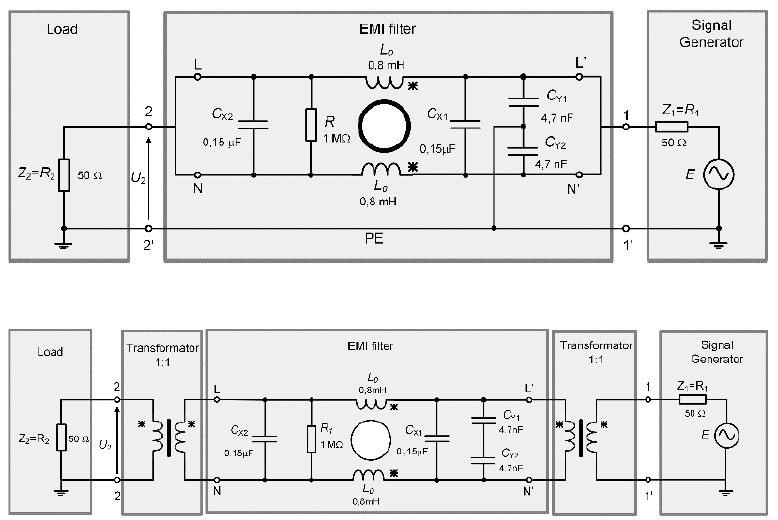
\includegraphics[width=10cm]{titelBild.png}
\end{figure}
\vfill

{
\renewcommand\arraystretch{2}
\begin{center}
\begin{tabular}{ >{\bf} l p{10cm} l }
Hochschule&Hochschule für Technik - FHNW\\
Studiengang&Elektro- und Informationstechnik\\
Auftraggeber&Dr. Luca Dalessandro\\
Betreuer&Prof. Dr. Sebastian Gaulocher \newline Prof. Peter Niklaus \newline Prof. Dr. Richard Gut \newline  Dr. Anita Gertiser \newline Pascal Buchschacher \\
Autoren&\textbf{Gruppe 1} \newline Niklaus Schwegler \newline Lukas von Däniken \newline Pascal Puschmann  \newline Simon Rohrer \newline Marco Binder\\
Version&2.0 %Normally not used!
\end{tabular}
\end{center}
}

\clearpage

			

%%---ABSTRACT----------------------------------------------------------------------------
\selectlanguage{ngerman}                %ngerman or english
\thispagestyle{empty}
\begin{abstract}
Die Firma Schaffner entwickelt EMI-Filter. Um diese zu modellieren benötigen sie eine Simulationssoftware. Die Hauptanwendung dieser Software besteht darin, die Einfügedämpfung, in Abhängigkeit der parasitären Parameter, über ein Frequenzspektrum bis 30Mhz zu visualisieren. Die Software sollte Plattformunabhängig und Modular erweiterbar sein. Daher wurde Java als Sprache verwendet. Als Grundstruktur dient die Model-View-Controller. Für die Berechnung wurden jeweils vereinfachte Ersatzschaltungen für Gleich- und Gegentaktstörungen modelliert. Die einzelnen Bauteile wurden modular in die Software implementiert. Durch eine kaskadierung wurden die Schaltungen nachgebaut und erzeugen somit die Simulationen. Auf der Benutzeroberfläche wurden für alle verstellbaren Parameter Slider erzeugt um die Werte um +-30\% zu verändern. Dabei werden die Auswirkungen für beide Signale direkt in zwei einzelnen Plots sichtbar. Die Software ist in der Lage Filter direkt miteinander zu vergleichen. Sie kann zudem einfach auf andere Schaltbilder erweitert werden. 

%lol wieso hetts do en iizug am aafang??????


\end{abstract}
\clearpage
%%---TABLE OF CONTENTS-------------------------------------------------------------------
\pagenumbering{Roman}
\selectlanguage{ngerman}                %ngerman or english
\tableofcontents
\clearpage
%%---TEXT--------------------------------------------------------------------------------
\pagenumbering{arabic}

\section{Einleitung} \label{sec:einleitung}
Entwurf Einleitung P2 EMI-Filter Team 1

Gemäss des Lastenhefts wurde der Auftrag erteilt, eine Simulationssoftware zu entwickeln. Diese Simulationssoftware soll die Einfügedämpfung eines EMI-Filters simulieren und grafisch darstellen. EMI-Filter werden üblicherweise in Schaltnetzteile verbaut, um zu verhindern, dass Störungen zurück ins Netz gespeist werden. Netzgeräte können unter Umständen hohe Frequenzen erzeugen, die sich nicht gut mit der Netzfrequenz von 50 Hz vertragen. Der EMI-Filter filtert genau diese hochfrequenten Signale heraus, um zu verhindern, dass andere Geräte, die auch ans Netz angeschlossen werden, nicht davon beeinträchtigt werden.

Um die Einfügedämpfung zu ermitteln, soll das EMI-Filter bezüglich der Gleich- und Gegentaktschaltung untersucht werden. Dies geschieht anhand zweier Funktionen für Gleich- und Gegentaktschaltung. Die Funktionen zeigen die Einfügdämpfung für einen Frequenzbereich bis 30MHz.Die beiden Schaltungen beinhalten die parasitären Parameter der elektrischen Komponenten, sodass eine möglichst wahrheitsgetreue Simulation gemacht werden kann. Die entwickelte Software soll die Einfügedämpfung grafisch darstellen.  Die Resultate werden für die Gleich- und Gegentaktschaltung in separaten Funktionen dargestellt. Des Weiteren sollen die elektrischen Komponenten der Schaltungen in der Simulationssoftware variiert werden können.
 
Damit sichergestellt werden kann, dass die Simulationen mathematisch korrekt sind, werden alle Berechnungen zuerst in MATLAB durchgerechnet. Diese Ergebnisse werden mit Simulationen der Simulationssoftware MPLAB MINDI verglichen. Des Weiteren wird überprüft, wie die Schaltung vereinfacht werden kann. Dies erfolgt einerseits durch Symmetrien der Schaltung, was dazu führt, dass Komponenten zusammengefasst werden können. Andererseits auch durch Weglassen aufgrund von vernachlässigbarem Einfluss auf die Simulationen. Die Softwarestruktur orientiert sich am gängigen Prinzip der MVC(Model-View-Control). Diese Strukturierung begünstigt einen modularen Aufbau, was die Software einfach erweiterbar macht und zudem eine unkomplizierte Wartung ermöglicht. Des Weiteren wird die Software anhand des Testkonzepts Modul für Modul getestet.

Im Fokus des Fachberichts befindet sich die Software, da das zu entwickelnde Produkt eine Simulationssoftware ist. Der Fachbericht ist nach dem Top-Down-Prinzip aufgebaut. In einem ersten Schritt wird die Software als Ganzes Beschrieben. In den darauffolgenden Kapiteln befinden sich die Dokumentationen der beiden Teile der Software. Die Software wird aufgegliedert in den Teil Benutzeroberfläche und den Teil Ermittlung der Einfügedämpfung. Um den Fachbericht schlank zu gestalten, werden sämtliche theoretische Grundlagen im Anhang platziert. Falls in Kapiteln entsprechende Theorie wichtig ist wird darauf verwiesen.


\section{Grundlagen} \label{sec:grundlagen}

\subsection{Elektrotechnik} \label{subsec:elektrotechnik}

\subsubsection{Aufbau eines EMI-Filters} \label{subsubsec:emi_filter}
Ein EMI-Filter ist ein lineares Netzwerk aus R, L, C Bauteilen und einem Transformator. Somit besitzten sie eine reziproke Übertragungssymetrie, was eine einfache Berechnungen von verschiedenen Zusammenhängen erlaubt. Einem reziproken Netzwerk ist die Betriebsrichtung gleichgültig.
Die Schaltung \ref{fig:orig_Schaltung} \nameref{fig:orig_Schaltung} zeigt den Filteraufbau, wie er der Aufgabenstellung zu entnehmen ist. Um das Gegentaktrauschen und das Gleichtaktrauschen bestimmen zu können, werden die beiden Schaltungsäquivalente gebildet. 

\begin{figure}[H]
	\centering
	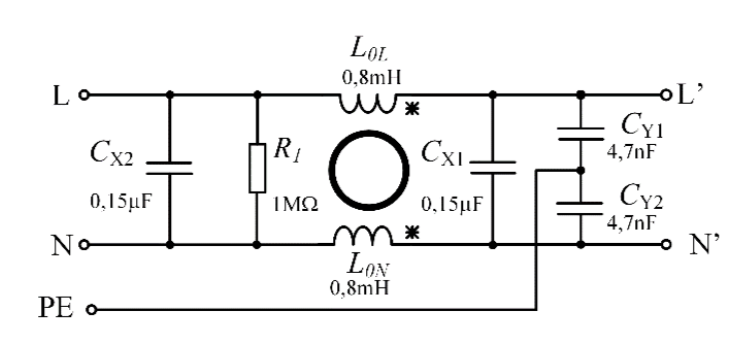
\includegraphics[width = 10cm]{orig_ElectricalCircuit.png}
	\caption{Original Schaltung \cite{aufgabenstellung}}
	\label{fig:orig_Schaltung}
\end{figure}


%TODO Die Schaltungsäquivalenzen müssen aufgeteilt werden und in die jeweiligen subsubsections gekippt werden
%TODO Reziprokzität einfügen
%TODO Allgemein EMI-Filter beschreiben

\subsubsection{Parasitäre Paramter}\label{subsec:parasitparam}
In diesem Unterkapitel werden grundsätzlich die Einflüsse und Eigenschaften von Parasitären Paramentern in Realen Bauteilen, besonders Spule und Kondensator, erklärt.

Ideale Bauteile beschreiben eine Funktion. Da reale Bauteile aus Materialien mit physikalischen Eigenschaften bestehen, treten bei der Umsetzung dieser Funktion Nebeneffekte auf. Sie entstehen, weil die einzelnen Bauteile im Betrieb elektrische Felder oder Magnetfelder erzeugen. Oder einfach durch die Leitfähigkeit eines Materials. Diese physikalisch bedingten Effekte werden als parasitär bezeichnet. Sie treten als Widerstand, Induktivität oder Kapazivität auf. Da sie gut klassifiziert werden können, werden sie als Parameter bezeichnet. 
Um eine Schaltung präzise zu simulieren ist es unerlässlich, die elektrischen Bauelemente mit den passenden parasitären Parametern zu ergänzen. In den Abbildungen \ref{fig:stray_L} und \ref{fig:stray_C} werden die parasitären Parameter von Spule und Kondensator gezeigt. Man stellt sie als zusätzliche Bauteile dar. \textcolor{red}{\textbf{TODO:Quelle ganzes kapitel}}


\begin{figure}[H]
	\begin{minipage}[h]{0.45\linewidth}
		\centering
		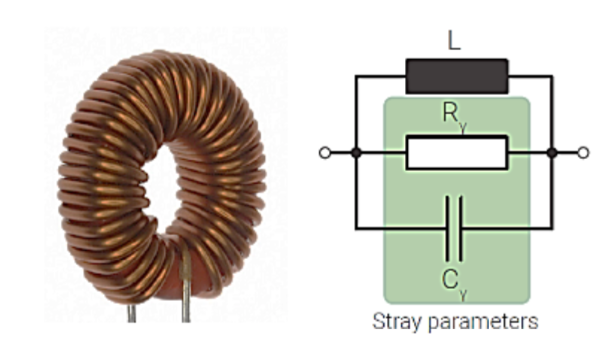
\includegraphics[width = 5cm]{stray_L.png}
		\caption{Parasiäre Elemente einer Induktivität \cite{aufgabenstellung}}
		\label{fig:stray_L}
	\end{minipage}	
	\begin{minipage}[h]{0.45\linewidth}
		\centering
		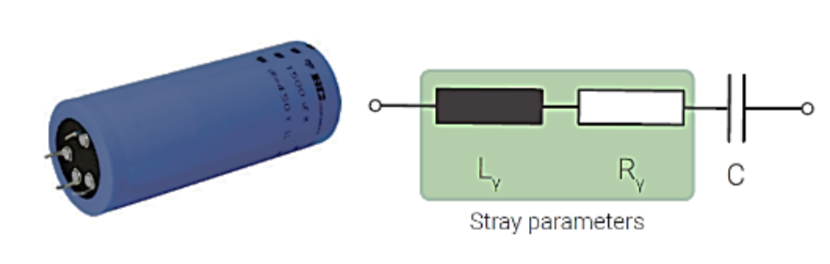
\includegraphics[width = 7cm]{stray_C.png}
		\caption{Parasiäre Elemente einer Kapazität \cite{aufgabenstellung}}
		\label{fig:stray_C}
	\end{minipage}
\end{figure}

\bigskip

\subsubsection{Gleich- Gegentaktschaltung} \label{subsubsec:gegentakt}

Dieses Kapitel basiert auf der Quelle \cite{p._niklaus_2-tore_2019}. In der realen Stromverteilung wird beabsichtigt, dass der Stromfluss über einen Zuleiter zum Verbraucher hinein-, respektive über einen Ableiter herausgeführt wird. 
Diese Art der Signalübertragung wird als Gegentakt-Betrieb bezeichnet. Im realen Stromnetz ist allerdings auch der sogenannte Gleichtakt-Betrieb vorhanden. Dabei wirken alle Leiter als Zuleiter, der gesamte Strom wird durch die Erde weggeleitet. Durch das Gesetz der Superposition ist es möglich, den Gleich- und den Gegentaktanteil getrennt voneinander zu betrachten. Dieses Phänomen wird in der Abbildung \ref{fig:auftrennen_der_leitung} dargestellt.  

\begin{figure}[H]
	\centering
	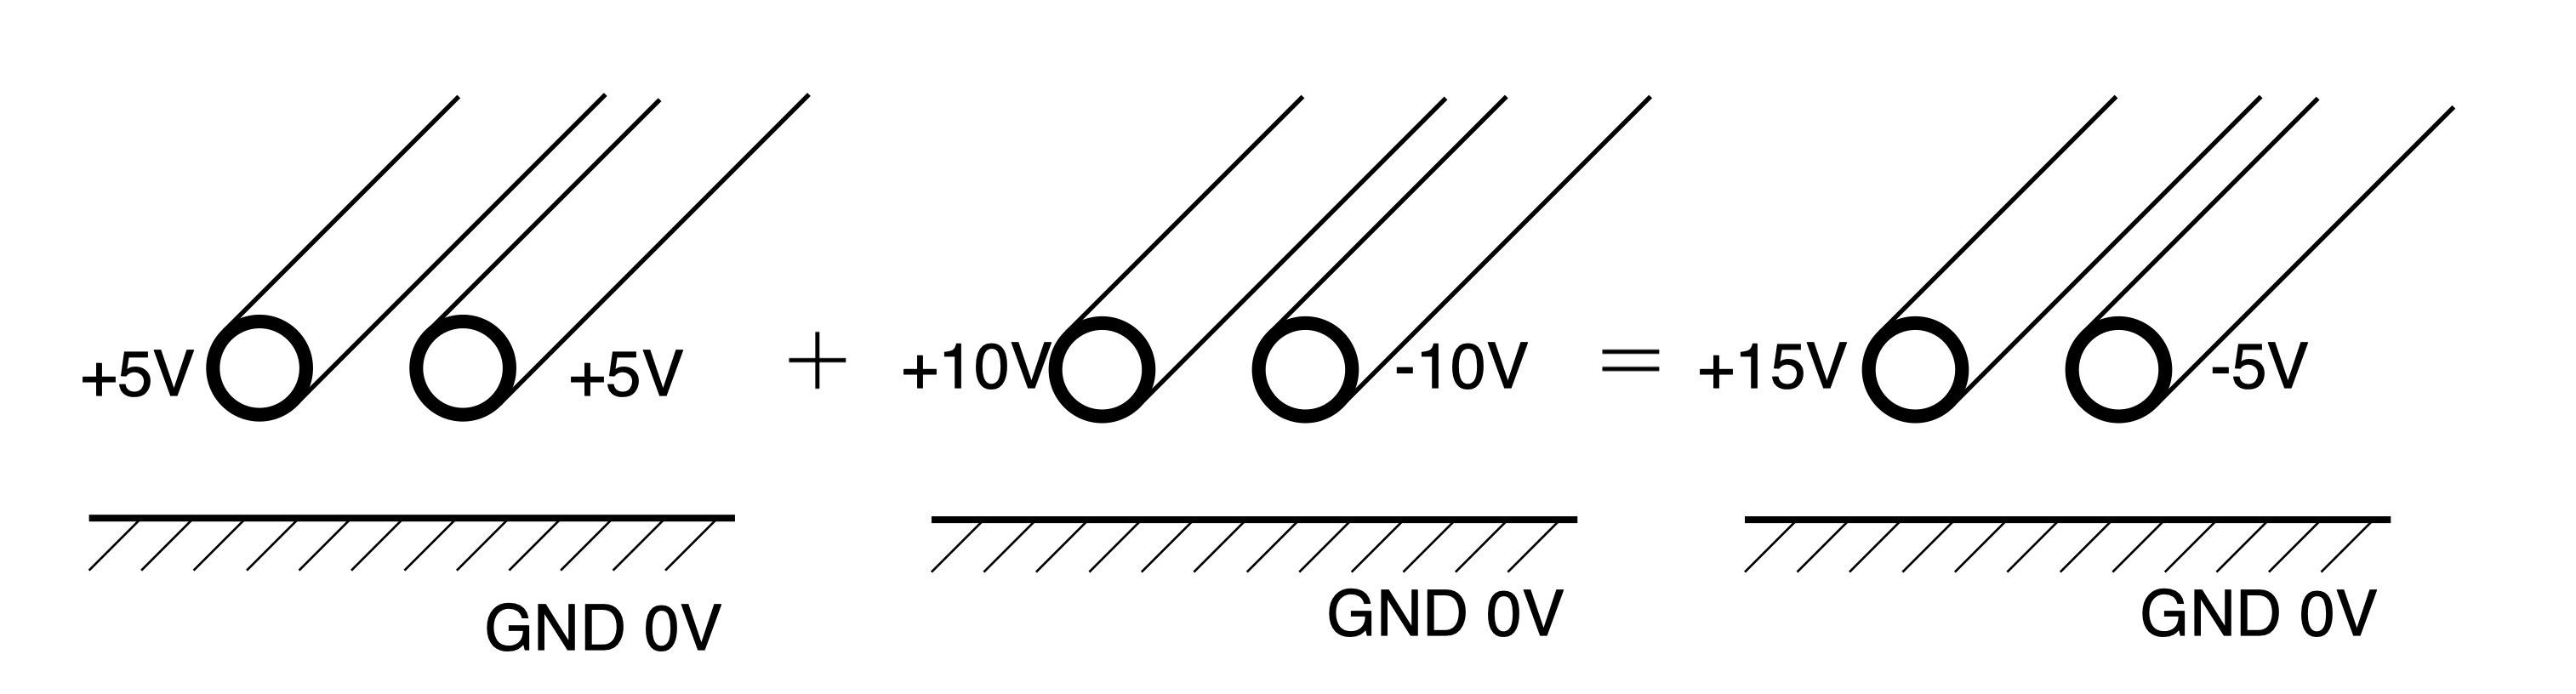
\includegraphics[width=15cm]{grundsatz_cm_dm.jpg}
	\caption{Beispiel aufgetrennten Leitung }
	\label{fig:auftrennen_der_leitung}
\end{figure} 


An einen geerdeten Verbraucher sind 2 Phasen angeschlossen. An der Zuleitung liegt eine Spannung von 15 Volt an, an der Rückleitung liegen -5 Volt an. Diese Leitung wird nun aufgeteilt in eine Gleichtaktleitung, bei welcher über beide Phasen 5 Volt eingespeist werden und in eine Gegentaktleitung, in welcher durch die Zuleitung 10 Volt, respektive in der Rückleitung -10V eingespiesen werden. Während in der Gleichtaktleitung die addierten 10 Volt gegenüber der Erde anliegen, werden sie in der Gegentaktleitung abgeführt. 


\newpage





\subsubsection{Einfügedämpfung}\label{subsec:einfuge}


 Um die Einfügungsverluste bestimmen zu können, wird das Model der 2-Tore verwendet. Einzelne Schaltungsteile werden in ABCD-Matrizen \ref{ABCD-Matrix} abgebildet, welche dann durch Kaskadierung der einzelnen ABCD-Matrixen zusammengeführt werden. Die Einfügungsverluste werden aus den Streuparameter\ref{subsec:Streuparameter} abgeleitet, welche direkt aus der ABCD-Matrix berechnet werden.




\subsubsection{Kettenmatrix}\label{subsubsec:kettenmatrix}
Folgendes Kapitel erklärt die Grundlagen der Kettenmatrix. Die Grundlagen basieren auf den Quellen \cite{hftech}\cite{Bernstein2015}.
Die Kettenmatrix ist eine Variante, um das Verhalten von 2-Toren zu beschreiben. Andere Varianten sind die Z-Matrix oder die Y-Matrix. Die Kettenmatrix hat jedoch den Vorteil, dass man in Serie geschaltene 2-Tore ohne grossen Aufwand zusammen rechnen kann. Sobald man die einzelnen Kettenmatrizen gebildet hat und die Schaltung soweit vereinfacht ist, dass nur noch in Serie geschaltene Ketten-Matrizen vorzufinden sind, können diese miteinander multipliziert werden. Das Matrix-Produkt stellt dann die Kettenmatrix der Gesamtschaltung dar. Folgende gängige Schaltungen helfen, die Kettenmatrizen der einzelnen Schaltungsteilen zu bilden (siehe Anhang: 2-Tor Tabellen).

Die Längsimpedanz lässt sich anhand der Kettenmatrix A\textsubscript{L} (Formel \ref{equ:horizImpedance}) darstellen
\begin{figure}[H]
	\begin{minipage}[h]{0.45\linewidth}
		\centering
		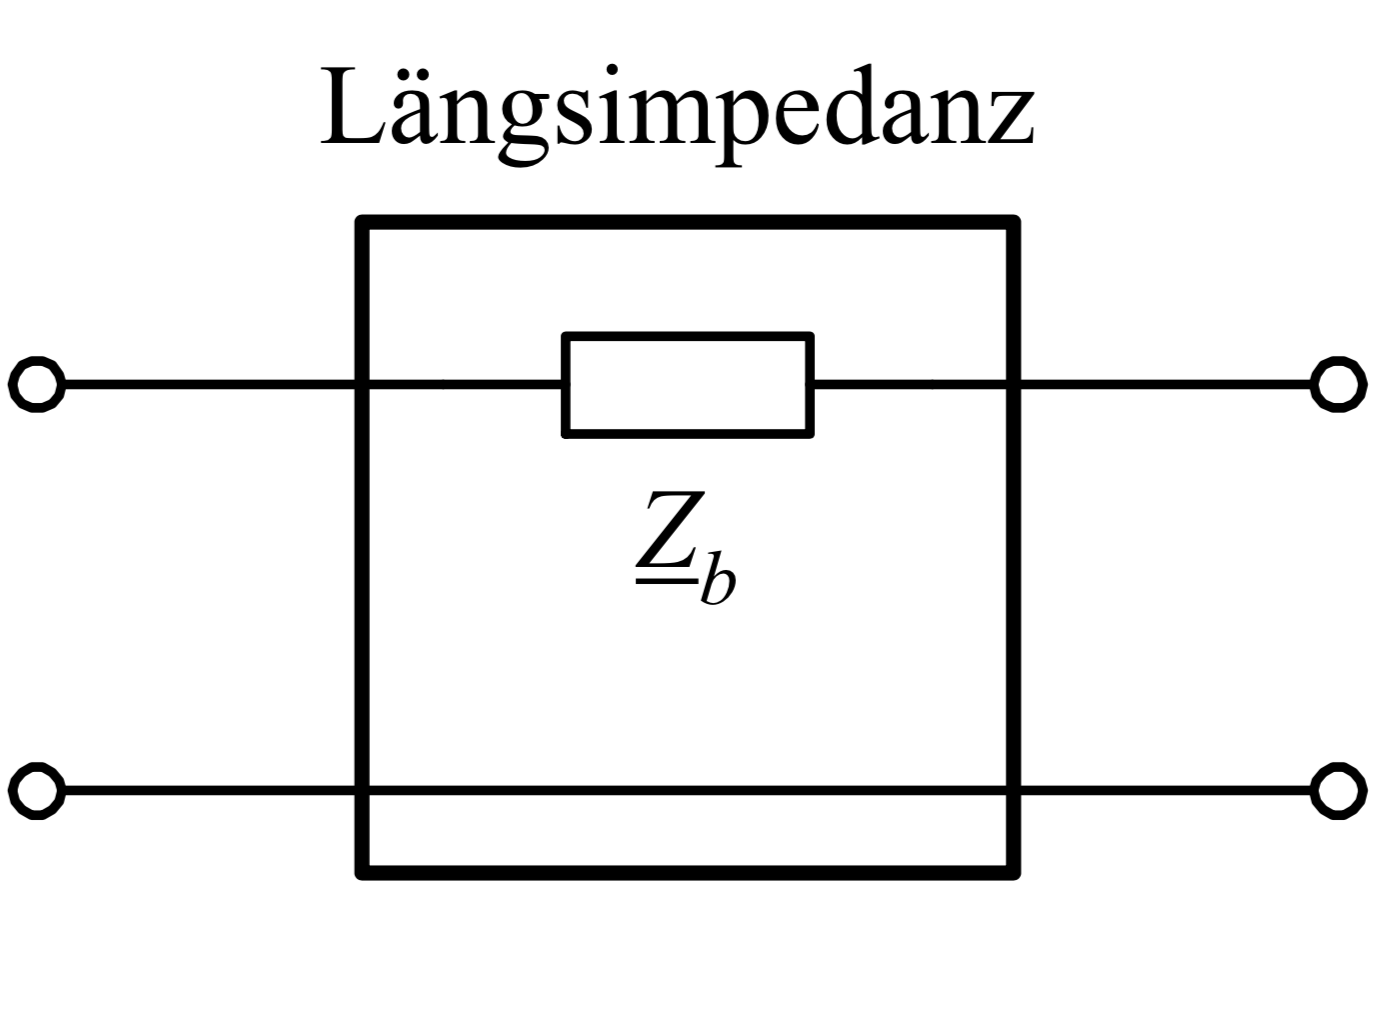
\includegraphics[width = 3cm]{h_impedance.png}
		\caption{Längsimpedanz \ref{sec:anhang}}
	\end{minipage}
	\begin{minipage}[h]{0.45\linewidth}
		\centering
		\begin{equation}\label{equ:horizImpedance}
			A_L = \left[\begin{matrix}
			1&\underline{Z}_b\\0&1
			\end{matrix}\right]
		\end{equation}
	\end{minipage}
\end{figure}

Die Querimpedanz lässt sich anhand der Kettenmatrix A\textsubscript{Q} (Formel \ref{equ:verticImpedance}) darstellen

\begin{figure}[H]
	\begin{minipage}[h]{0.45\linewidth}
		\centering
		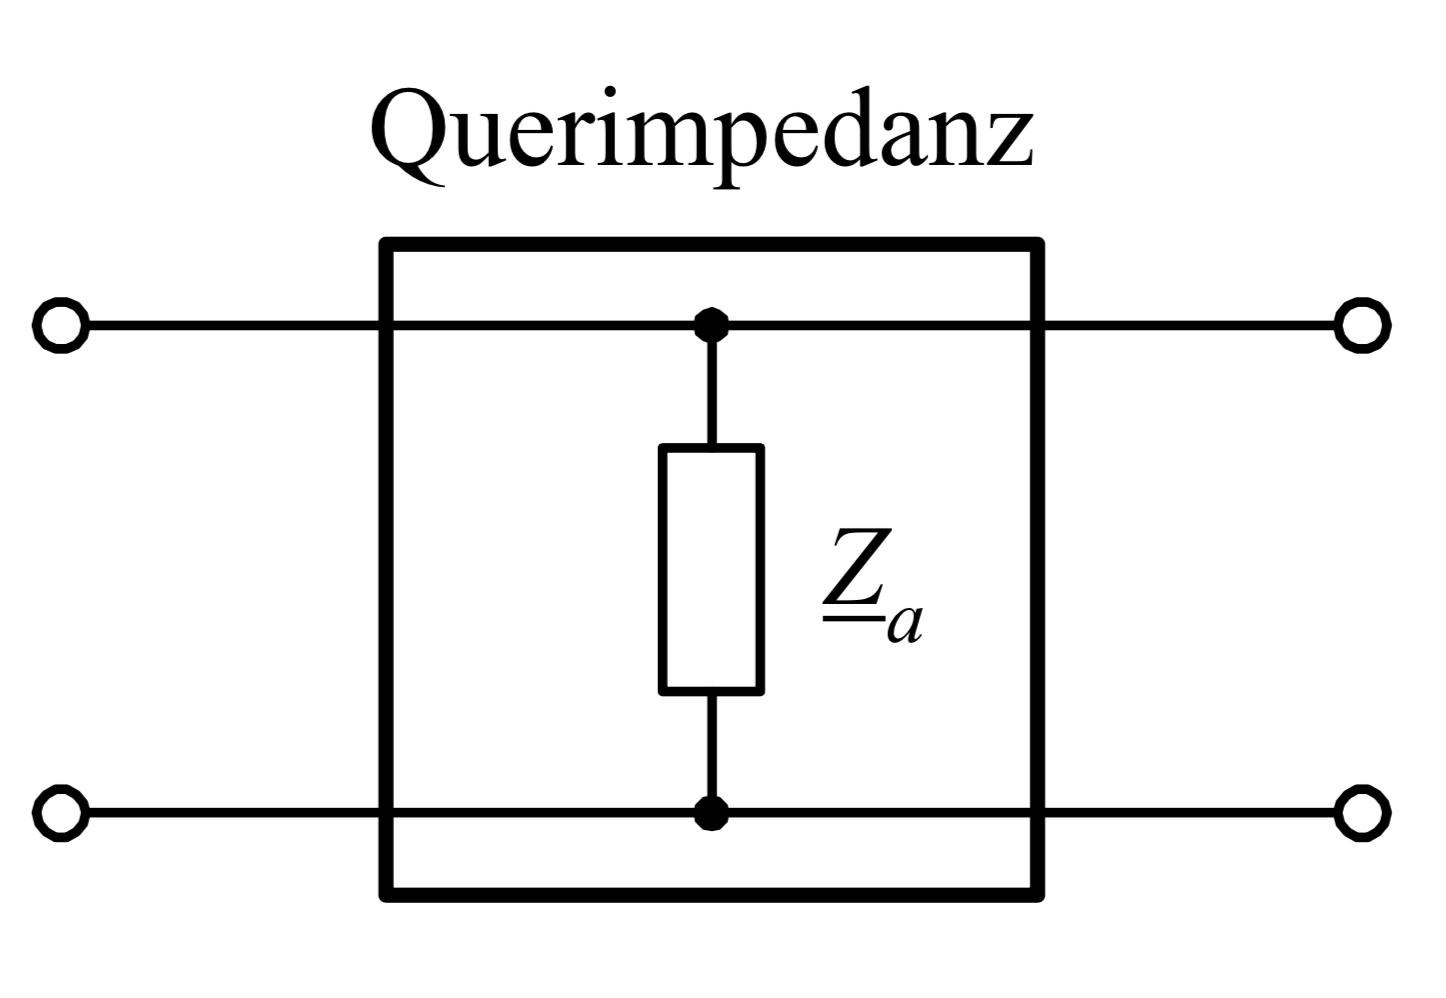
\includegraphics[width = 3cm]{v_impedance.png}
		\caption{Querimpedanz \ref{sec:anhang}}
	\end{minipage}
	\begin{minipage}[h]{0.45\linewidth}
		\centering
		\begin{equation}\label{equ:verticImpedance}
			A_Q = \left[\begin{matrix}
			1&0\\\frac{1}{\underline{Z}_a}&1
			\end{matrix}\right]
		\end{equation}
	\end{minipage}
\end{figure}


Sobald die Kettenmatrix einer Schaltung gebildet wurde, kann diese direkt in die Streuparameter umgewandelt werden. Der $s_{21}$ Parameter kann wie in Formel \ref{equ:s21} beschrieben, durch Einsetzen der Kettenmatrix bestimmt werden. Für den Widerstand $R_w$ muss die verwendete Bezugsimpedanz eingesetzt werden.
\begin{equation}\label{equ:s21}
s_{21} = \frac{2}{A_{11}+\frac{A{12}}{R_w}+A_{21}*R_w+A_{22}}
\end{equation}
Die Indexierung der Kettenmatrix wird in der Formel \ref{equ:A_index} gezeigt.
\begin{equation}\label{equ:A_index}
	A = \left[\begin{matrix}
	A_{11}&A_{12}\\A_{21}&A_{22}
	\end{matrix}\right]
\end{equation}
\newpage



\subsection{Programmieren} \label{subsec:softech}
\subsubsection{MVC-Struktur}\label{subsec:mvc}

Das MVC-Framework wird zur Softwarestrukturierung verwendet. Durch diese Strukturierung werden die Berechnungen der Daten (eng. model), die Steuerung (engl. controller) und dessen graphischer Repräsentation (engl. view) getrennt. In der Abbildung (TODO) ist dieser Aufbau in einem Beispielklassendiagramm dargestellt.

%TODO Bild Gut MVC

Der Ablauf dieser Struktur ist wie folgt: 

\begin{enumerate}
\item Benutzereingabe löst Event aus
\item Die Aktion wird dem Controller übergeben. Dieser holt die Daten in der View, leitet diese dem Model weiter und löst die Berechnungen aus
\item Das Model führt die Berechnungen aus und informiert den Observer
\item Das Model führt die Berechnungen aus und informiert den Observer
\item Der Observer löst ein Event in der View aus. View kann die Daten vom Model holen und Ausgeben
\end{enumerate}




\section{Ermitteln der Einfügedämpfung} \label{sec:umsetzung}
In diesem Kapitel wird ausführlich beschrieben, wie aus den gegebenen Gleich- und Gegentaktschaltung (Verweis Aufgabenstellung) die Einfügedämpfung ermittelt wird. Um die einzelnen Schritte konsistent zu beschriebenen, wird an den entsprechenden Stellen Bezug auf die theoretischen Grundlagen Kapitel \ref{sec:Grundlagen} genommen. Der erste Abschnitt behandelt die Gleichtaktschaltung \ref{subsec:zusammenfassungGleichtakt} und in einem zweiten Abschnitt wird die Gegentaktschaltung \ref{subsec:zusammenfassungGegentakt} behandelt. In diesen beiden Kapitel wird beschrieben, wie aus den Schaltungen aus der Aufgabenstellung die Kettenmatrizen der beiden Schaltungen ermittelt wird. Aus der Kettenmatrix kann somit die Einfügedämpfung berechnet werden, wie in Kapitel \ref{subsec:subsec:einfuge} beschrieben.


\subsection{Gleichtaktschaltung}\label{subsec:zusammenfassungGleichtakt}
Um die Einfügedämpfung zu ermitteln, wird im ersten Schritt die Schaltung weitgehend vereinfacht. Die reduzierte Schaltung wird anhand der Kettenmatrix (siehe \ref{subsec:Kettenmatrix}) beschrieben. Aus der Kettenmatrix wird dann für den vorgegebenen Frequenzbereich die Einfügedämpung berechnet.

\paragraph{Reduktion der Schaltung}\label{para:redukGleichtakt}
Abbildung \ref{fig:CMSchaltungOriginal} zeigt die Schaltung aus der Aufgabenstellung. 
\begin{figure}[H]
	\centering
	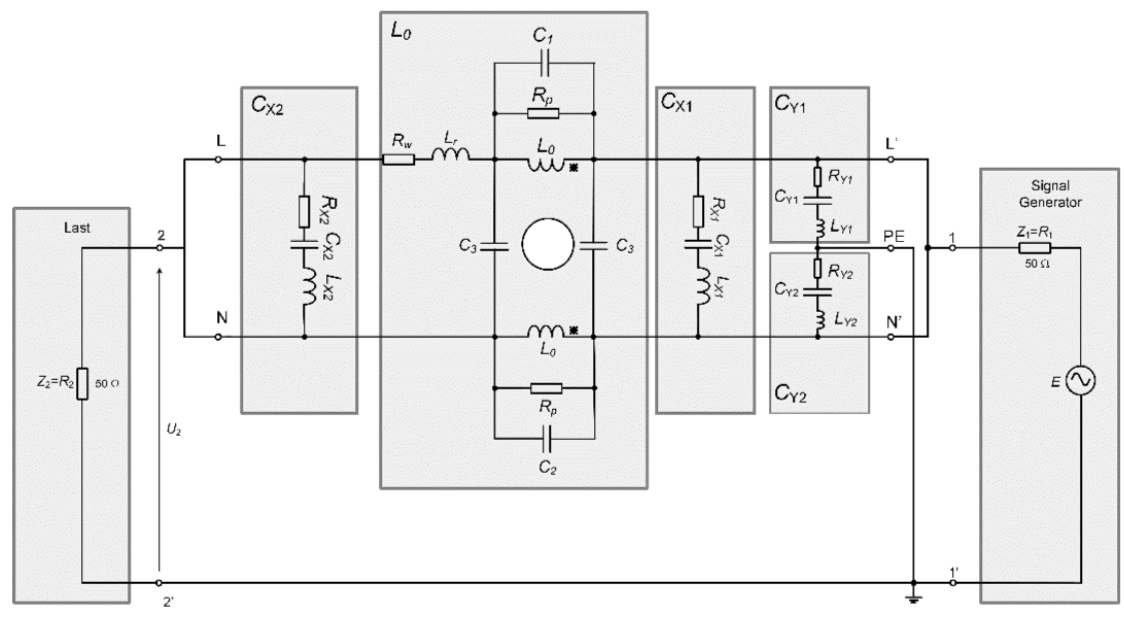
\includegraphics[width = 10cm]{CM_Aufgabenstellung.png}
	\caption{Originale Gleichtaktschaltung\cite{aufgabenstellung}}
	\label{fig:CMSchaltungOriginal}
\end{figure}
Die Originalschaltung wird mit den Komponenten $R_w$ und $L_r$ ergänzt, sodass sie symmetrisch ist. Dies macht es möglich, dass die Schaltung weiter vereinfacht werden kann. Zudem wurden $C_1$ und $C_2$ in $C_p$ und $C'_p$ umbenannt um zu zeigen, dass es sich um die gleiche Kapazität handelt. Durch weglassen des Eisenkerns, wird $L_0$ und $L'_0$ mit dem Vorfaktor zwei ergänzt da sich die Magnetfelder überlagern. %TODO besser schreiben%
Durch diese Änderungen ergibt sich die Schaltung in Abbildung \ref{fig:CMSchaltungErgänzt}.
\begin{figure}[H]
	\centering
	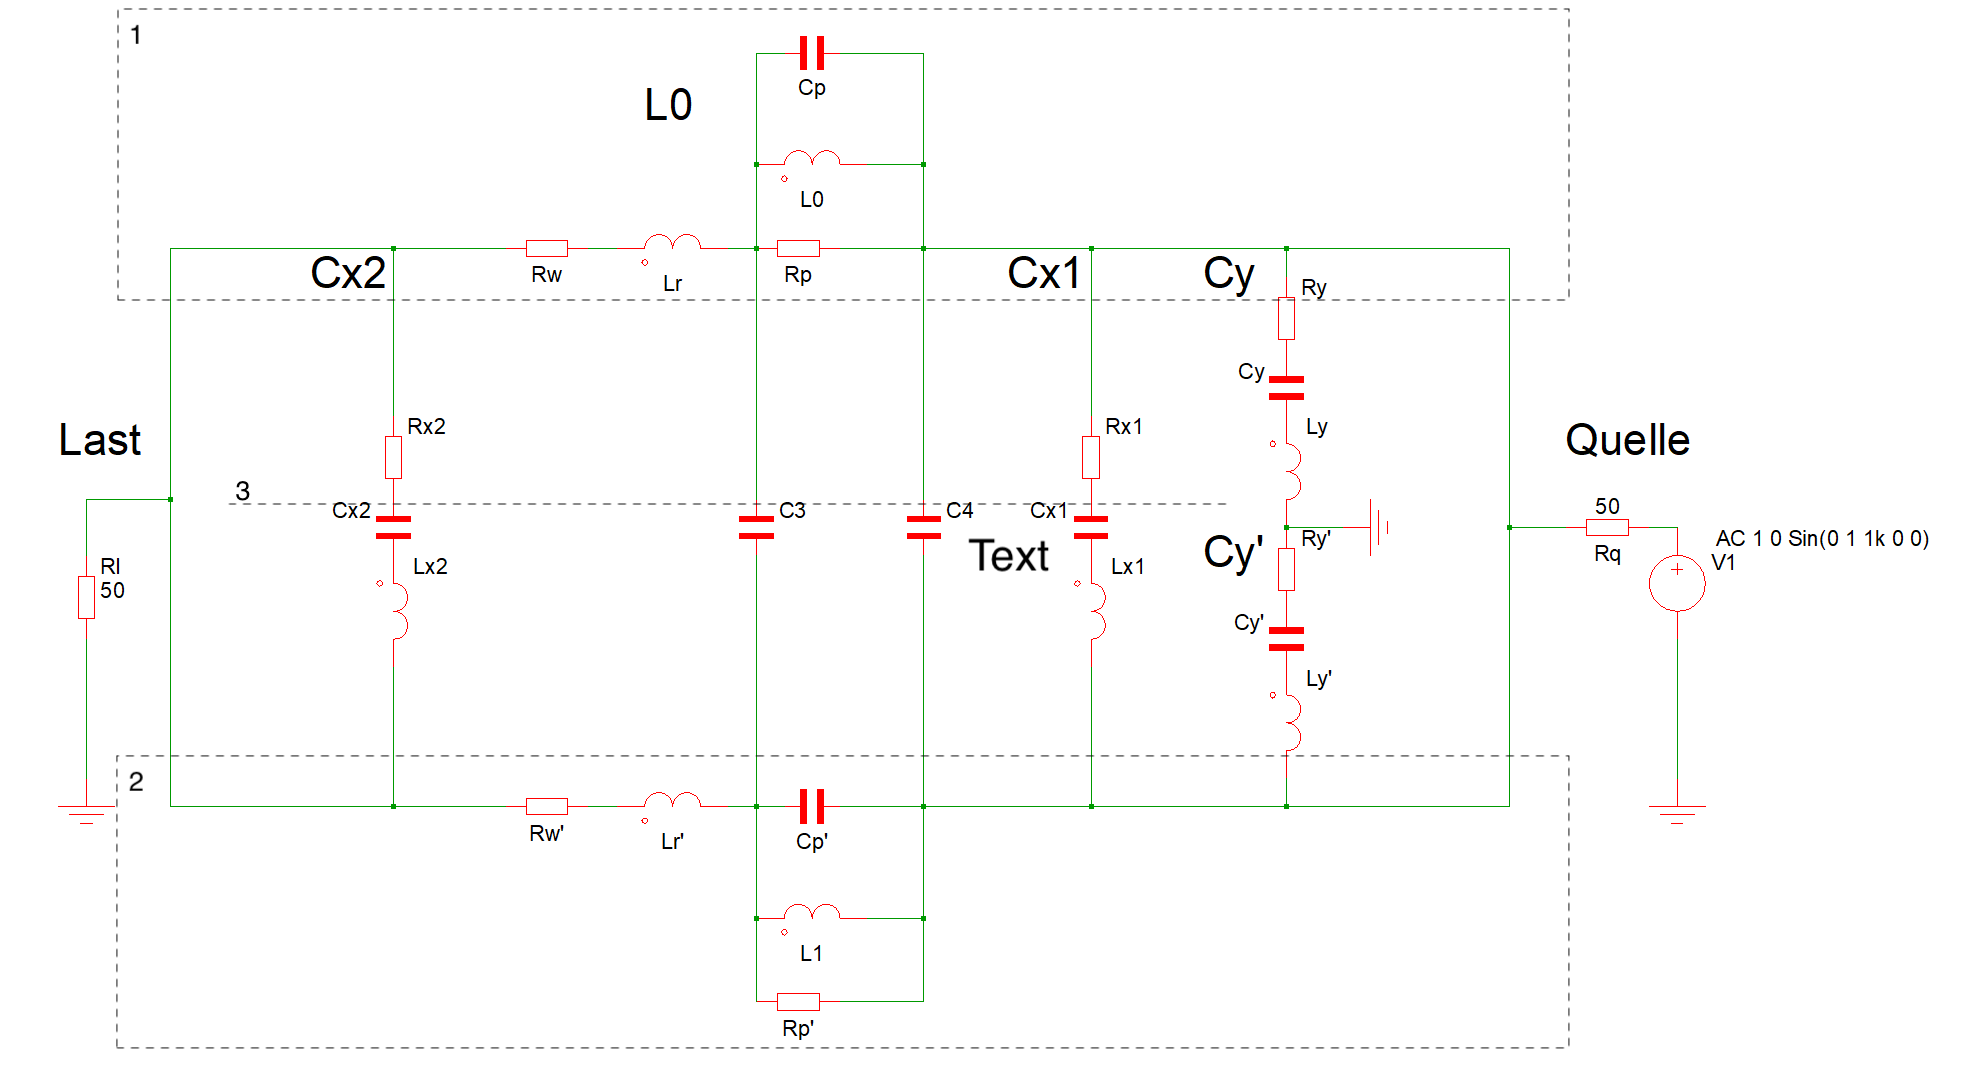
\includegraphics[width = 15cm]{EMI_CMpretty1.png}
	\caption{Ergänzte Gleichtaktschaltung}
	\label{fig:CMSchaltungErgänzt}
\end{figure}
 Der obere Strang(siehe Abbildung \ref{fig:CMSchaltungErgänzt}, Nr. 1) und untere Strang (siehe Abbildung \ref{fig:CMSchaltungErgänzt}, Nr. 2) sind identisch. Da es keinen Potentialunterschied zwischen ihnen gibt, kann die Schaltung entlang der Symmetrie-Achse (siehe Abbildung \ref{fig:CMSchaltungErgänzt}, Nr. 3) aufgetrennt werden. Dies ergibt die Schaltung in Abbildung \ref{fig:CMSchaltungaufgetrennt}.

\begin{figure}[H]
	\centering
	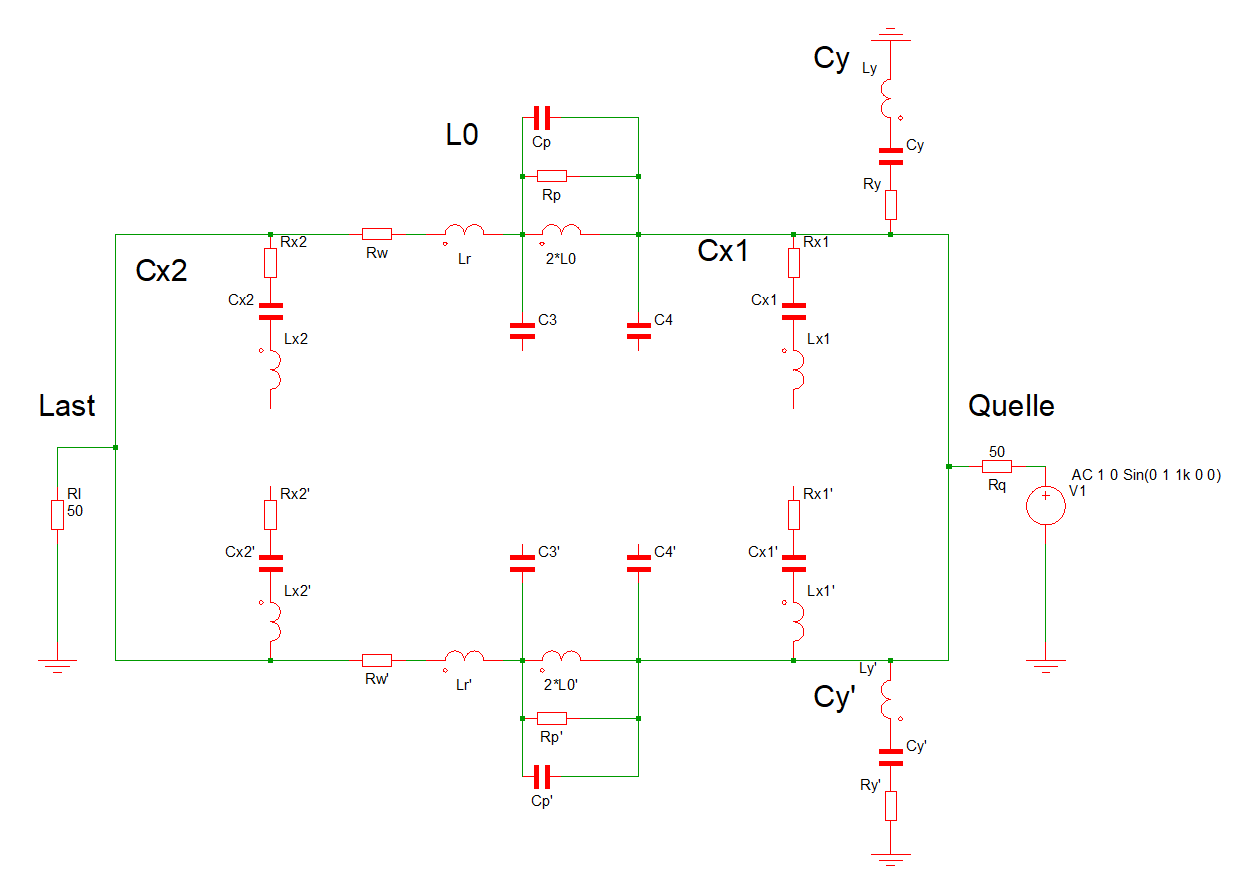
\includegraphics[width = 10cm]{EMI_CMpretty2.png}
	\caption{Aufgetrennte Gleichtaktschaltung}
	\label{fig:CMSchaltungaufgetrennt}
\end{figure}
Komponenten die nicht mehr fest verbunden sind, fallen weg. Dies gilt für die Kondensatoren $C_3$, $C_4$, $C_{x1}$ und $C_{x2}$. Die weiter reduzierte Schaltung wird in Abbildung \ref{fig:CMSchaltungvereinfacht1} abgebildet.
\begin{figure}[H]
	\centering
	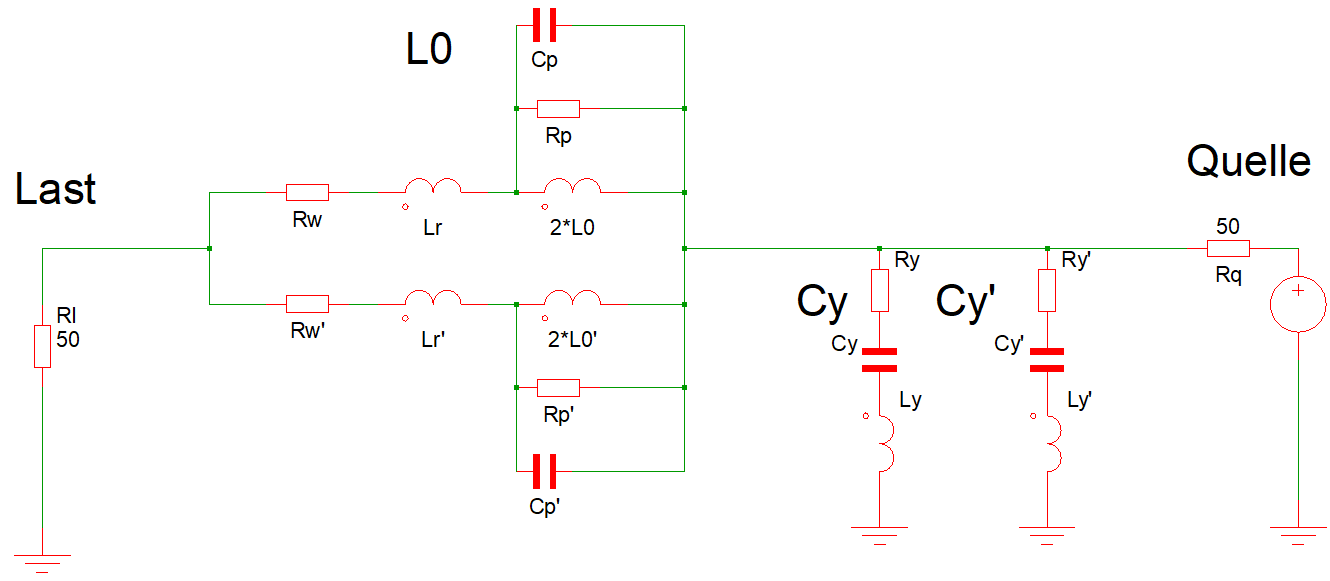
\includegraphics[width = 10cm]{EMI_CMpretty3.png}
	\caption{Vereinfachte Gleichtaktschaltung}
	\label{fig:CMSchaltungvereinfacht1}
\end{figure}
Die übrigen Komponenten von $L_0$ bilden eine Parallelschaltung, welche sich durch halbieren der Widerstände und Induktivitäten und verdoppeln der Kapazitäten zusammenfassen lässt. Zusätzlich werden die beiden $C_y$ und $C'_{y}$ parallel auf das Bezugspotential geschalten. Da $C_y$ und $C'_y$ identisch sind, werden sie wie in Abbildung \ref{fig:CMSchaltungvereinfacht} zusammengefasst. Diese vereinfachte Schaltung bildet die Grundlage für die Berechnungen der Software.

\begin{figure}[H]
	\centering
	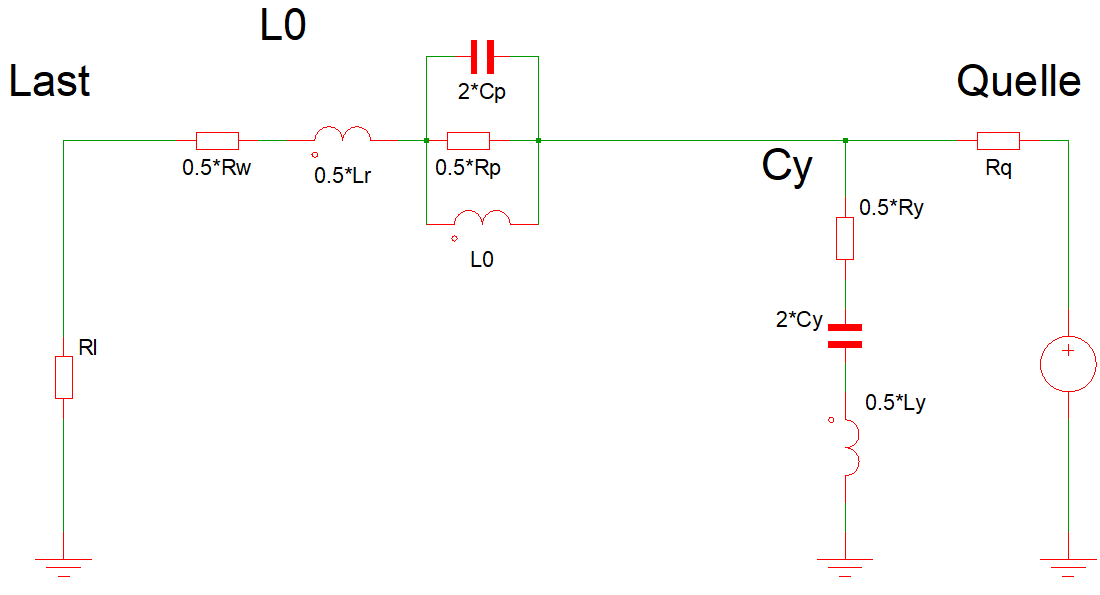
\includegraphics[width = 10cm]{EMI_CMpretty.png}
	\caption{komplett reduzierte Gleichtaktschaltung}
	\label{fig:CMSchaltungvereinfacht}
\end{figure}

\paragraph{Bilden der Kettenmatrix}\label{para:kettenGleichtakt}
Damit die Kettenmatrix der Gesamtschaltung gebildet werden kann, wird in einem ersten Schritt die reduzierte Schaltung in Längs- und Querimpedanzen (siehe Kapitel \ref{subsec:kettenmatrix} eingeteilt. Diese werden in Abbildung \ref{fig:cmschaltungEingeteilt} mit den Kennzeichnungen „QI“ und „LI“ vermerkt wobei „QI“ für Querimpedanz steht und „LI“ für Längsimpedanz. Die Impedanzen der einzelnen Schaltungsteile werden in die Kettenmatrizen für Quer- und Längsimpedanz eingesetzt. Die Kettenmatrizen werden durch Kaskadierung zur Kettenmatrix der Gesamtschaltung zusammengefasst.
\begin{figure}[H]
		\centering
		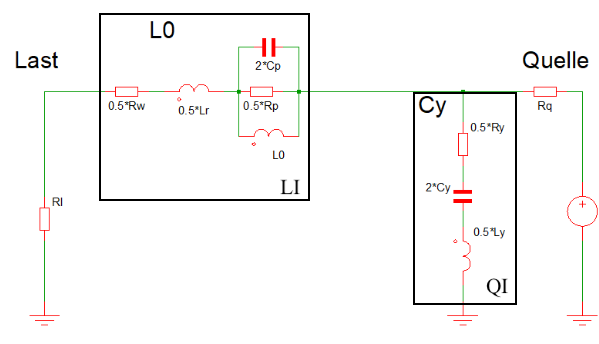
\includegraphics[width = 10cm]{EMI_CMvereinfacht_markiert.png}
		\label{fig:cmschaltungEingeteilt}
		\caption{Einteilung der Gleichtaktschaltungteile}
\end{figure}
Anhand der Kettenmatrix der Gesamtschaltung kann die Einfügedämpfung direkt ermittelt werden, indem mit der Formel \ref{equ:s21ausAMatrix} der Streuparameter $S_{21}$ berechnet wird(siehe Kapitel \ref{sec:einfuge}). $R_w$ ist die Bezugsimpedanz. Die Bezugsimpedanz bezieht sich auf die Innenimpedanz der Quelle und die Lastimpedanz. Bezüglich der Aufgabenstellung(Verweis Aufgabenstellung) ist dieser auf 50Ohm festgelegt.

\begin{equation}\label{equ:s21ausAMatrix}
s_{21} = \frac{2}{A_{11}+\frac{A{12}}{R_w}+A_{21}*R_w+A_{22}}
\end{equation}


\subsection{Gegentaktschaltung}\label{subsec:zusammenfassungGegentakt}
\paragraph{Reduktion der Schaltung}\label{para:redukGegentakt}
Folgender Abschnitt legt Schritt für Schritt dar, wie die Gegentaktschaltung vereinfacht wird. Die Abbildung \ref{fig:DMSchaltungAufgabenstellung} zeigt die Originalschaltung, wie Sie der Aufgabenstellung entnommen wurde. In einem ersten Schritt wird die gekoppelte Spule (Im Bild L0) vereinfacht. Die Magnetfelder der beiden Induktivitäten L0 kompensieren sich gegenseitig. Sie fallen weg, da sie Niederohmig werden. Somit verschwindet L0 mit den parasitären Elementen C1, C2 und die beiden Widerstände Rp.
\begin{figure}[H]
	\centering
	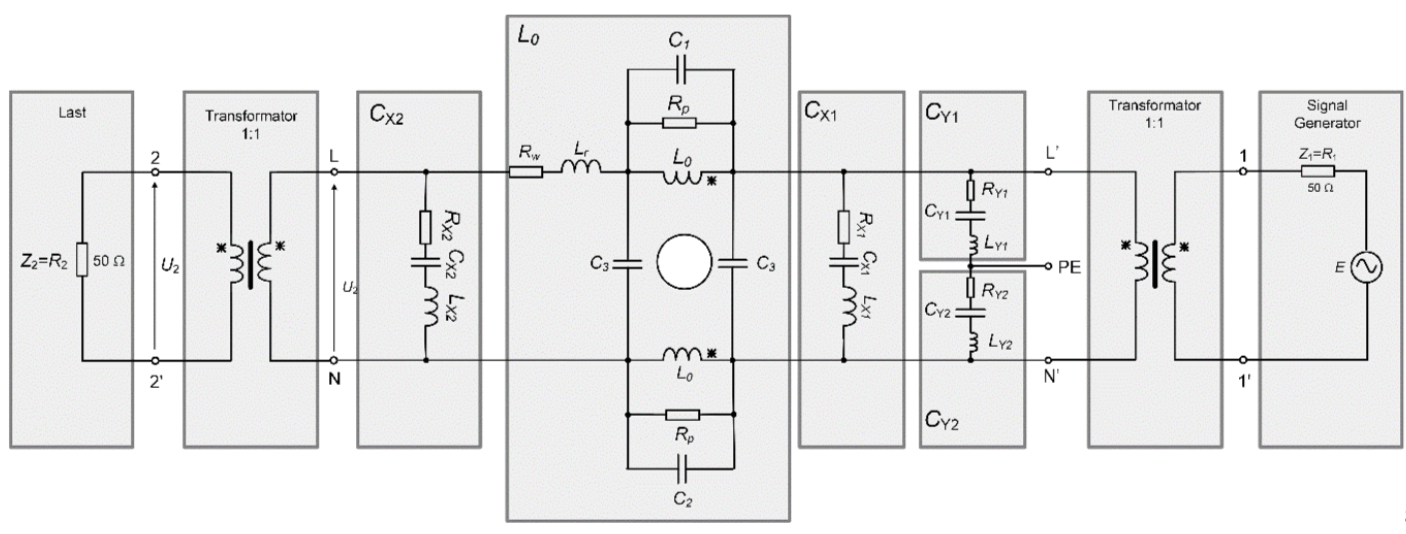
\includegraphics[width = 15cm]{DM_Aufgabenstellung.png}
	\caption{Originale Gegentaktschaltung}
	\label{fig:DMSchaltungAufgabenstellung}
\end{figure}
Durch diese Veränderungen erhält man die Gegentaktschaltung mit reduziertem L0(Abbildung \ref{fig:DMSchaltungreduziertL0}). Damit die Symmetrie der Schaltung gegeben ist, werden im unteren Strang Rw’ und Lw’ ergänzt. Diese Änderungen sind auch in der Gleichtaktschaltung vorhanden. Zudem werden die Kondensatoren C3 und C4 entfernt. Die Einflüsse sind aufgrund der kleinen Kapazität zu vernachlässigen. 
\begin{figure}[H]
	\centering
	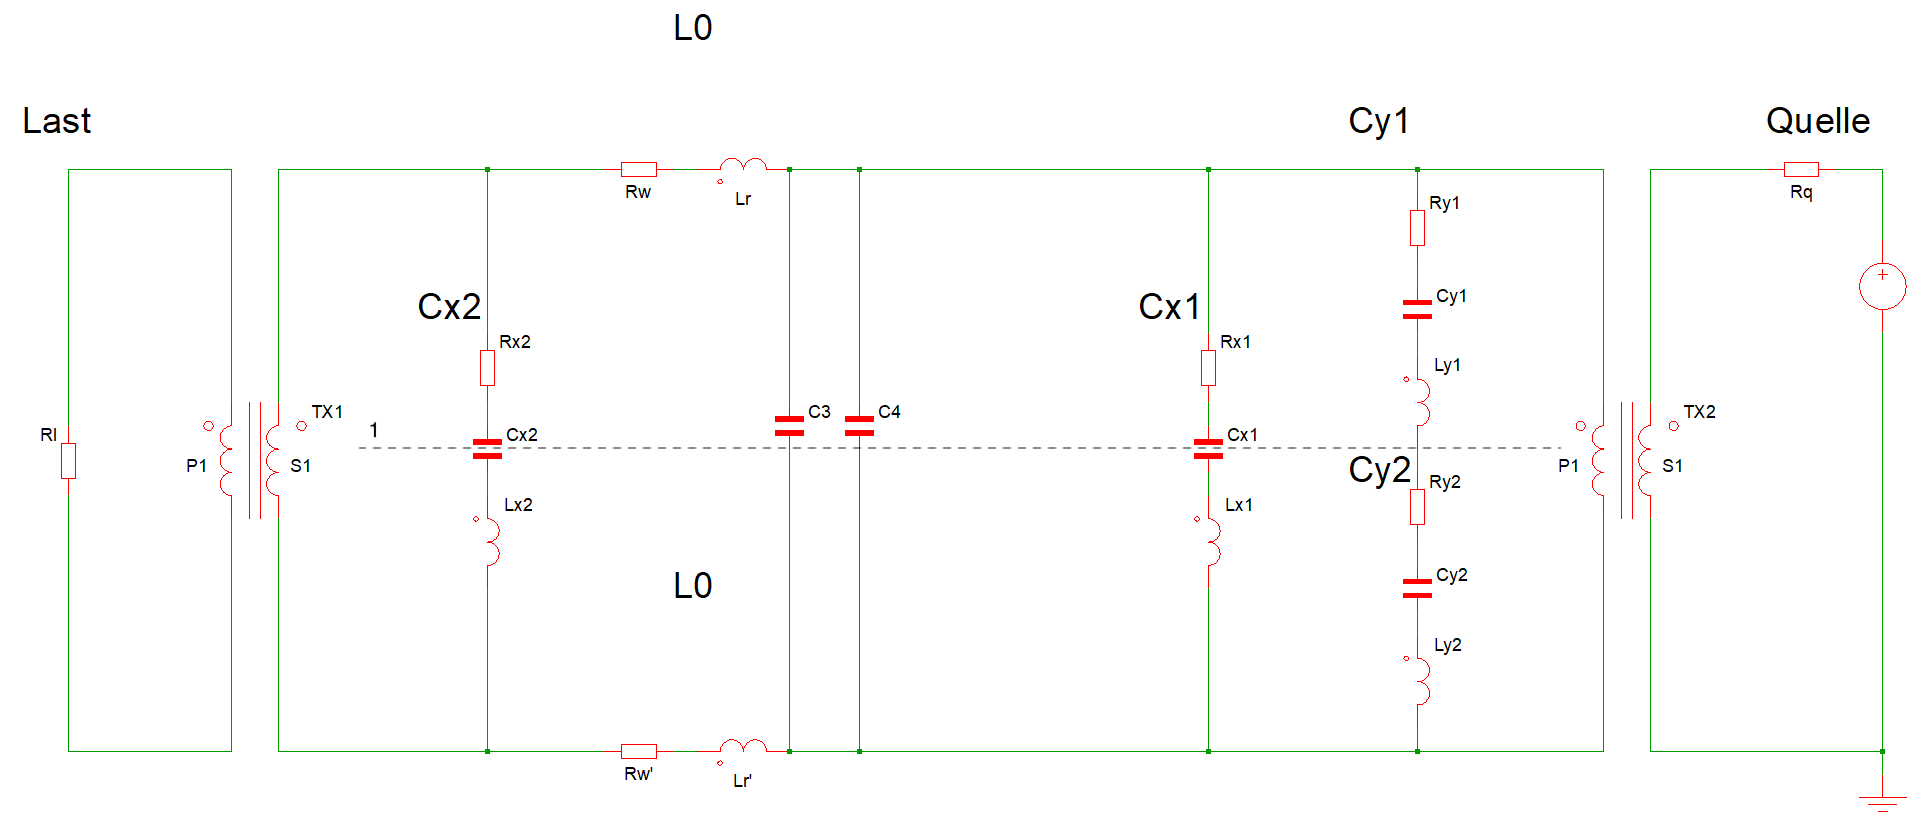
\includegraphics[width = 15cm]{EMI_DMpretty4.png}
	\caption{Gegentaktschaltung mit reduziertem L0}
	\label{fig:DMSchaltungreduziertL0}
\end{figure}
In einem nächsten Schritt wird mithilfe der Symmetrie der Schaltung weitere Teile zusammengefasst. Die im Bild eingezeichnete Linie(Abbildung \ref{fig:DMSchaltungreduziertL0}, Nr.1) entspricht der Symmetrie. Entlang dieser Linie werden die Verbindungen getrennt. Die offenen Enden werden auf das Bezugspotential geschalten. Dabei werden bei den aufgetrennten Verbindungen die elektrischen Komponenten aufgeteilt. Widerstände und Induktivitäten werden halbiert und die Kapazitäten verdoppelt. Durch dieses Vorgehen ergibt sich die Schaltung, wie in Abbildung \ref{fig:DMSchaltungSymAufgetrennt} ersichtlich.
\begin{figure}[H]
	\centering
	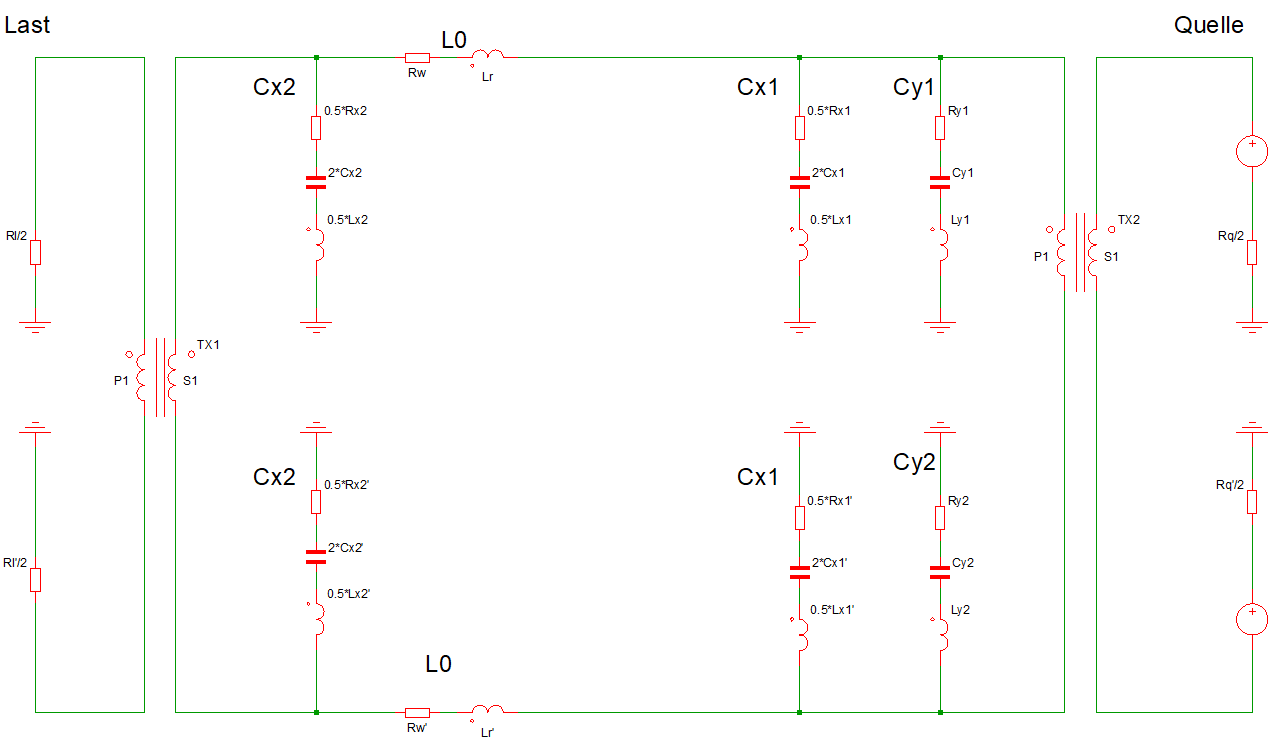
\includegraphics[width = 15cm]{EMI_DMpretty7.png}
	\caption{symmetrisch aufgetrennte Gegentaktschaltung}
	\label{fig:DMSchaltungSymAufgetrennt}
\end{figure}
Der obere und untere Teil der aufgetrennten Schaltung sind weitgehend identisch. Somit reduziert sich die Schaltung auf einen der beiden Stränge. Abbildung \ref{fig:DMSchaltungvereinfacht} zeigt die komplett vereinfachte Schaltung, welche die Grundlagen für die Gegentaktberechnungen bildet. 
\begin{figure}[H]
	\centering
	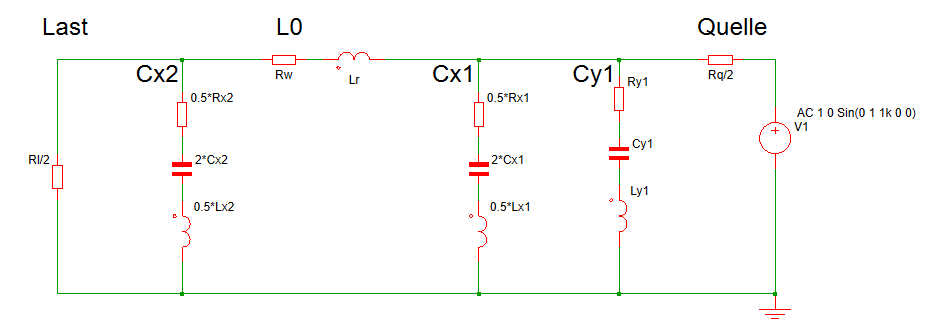
\includegraphics[width = 15cm]{EMI_DMvereinfacht.png}
	\caption{komplett vereinfachte Gegentaktschaltung}
	\label{fig:DMSchaltungvereinfacht}
\end{figure}

\paragraph{Bilden der Kettenmatrix}\label{para:kettenGegentakt}
Abbildung \ref{fig:dmschaltungEingeteilt} zeigt die Einteilung der reduzierten Schaltung in Längs- und Querimpedanzen.
 
\begin{figure}[H]
		\centering
		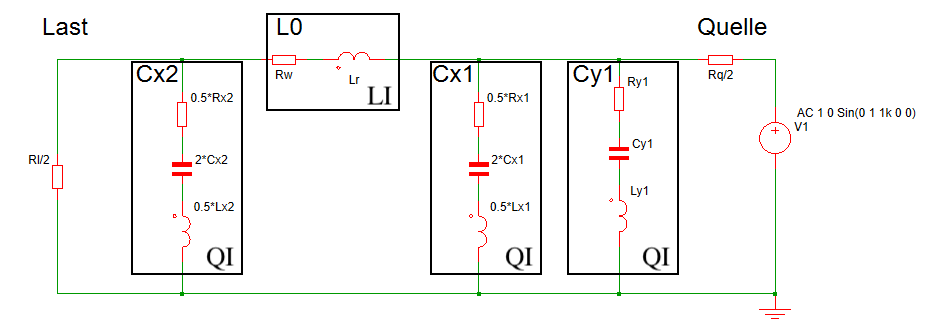
\includegraphics[width = 10cm]{EMI_DMvereinfacht_markiert.png}
		\label{fig:dmschaltungEingeteilt}
		\caption{Einteilung der Gegentaktschaltungsteile}
\end{figure}

Im nächsten Schritt werden die Impedanzen der einzelnen Schaltungsteile gebildet, welche in die passenden Kettenmatrizen eingesetzt werden.
Wiederum durch Kaskadierung der einzelenen Kettenmatrizen wird die Kettenmatrix der Gesamtschaltung gebildet. Aus der Kettenmatrix wird, wie bei der Gleichtaktschaltung die Einfügedämpfung berechnet. Ein wichtiger Unterschied ist jedoch, dass bei der reduzierten Gegentaktschaltung (Abbildung \ref{fig:DMSchaltungvereinfacht}) $R_w$ 25Ohm ist. 



\section{Software} \label{sec:software}

knackiger Top-Down beschrieb des IST-Zustands der fertigen software. 

Es werden stets Fachbegriffe verwendet. 


In dieser Section wird erklärt warum die Software wie aufgebaut ist.

Ebenfalls wird beschrieben welche berechnungen in welcher Klasse durchgeführt werden
Das heisst, dass wir hier auch Bilder der Vereinfachten Schaltung zeigen und wie wir diese Aufteilen in einzelne Glieder


\section{Testkonzept}\label{sec:testkonzept}
Wieso, weshalb und Warum
\subsection{Prinzip} \label{prinzip}
Wie ist das Testkonzept aufgebaut
\subsection{Validierung} \label{validierung}
Testergebnisse darstellen und Interpretieren

Ebenfalls wird hier beschrieben welche Werte wir mit der Simulation und mit Matlab erreicht haben

\section{Schluss} \label{sec:schluss}
Zum Abschluss des Projektes und nachdem alle Test durchgeführt wurden, wird die Software dem Auftraggeber zur Verfügung gestellt. Alle im Pflichtenheft gesteckte Muss-Ziele wurden zufriedenstellend umgesetzt. Die Software ist in der Lage die Eifügedämpfung eines EMI-Filters grafisch darzustellen. Ausserdem ist es möglich verschiedene Filterprofile anzulegen und sie zu speichern. Die verschieden Filter können gleichzeitig im Plot angezeigt werden. 

Die grösste Herausforderung während des Projektes bestand aus der Erarbeitung der elektrotechnischen Grundlagen und die Berechnung der Einfügedämpfung des Netzwerkes in DM und CM. Die Entwicklung des Softwaregrundgerüsts ging zügig vorwärts. Die Schwierigkeiten bei der Software waren beispielsweise die Implementierung der durchgeführten Berechnungen in den Code und die Verarbeitung der Werte, die in die GUI eingegeben werden. Um die Performence nicht einzuschränken, können nur 10 Filterprofile gleichzeitig angezeigt werden.

Schlussendlich konnten alle Schwierigkeiten gut gemeistert werden. Die Software könnte natürlich noch weiterentwickelt werden.  Eine weitere sinnvolle Funktion wäre eine Monte-Carlo Analyse. Diese wurde jedoch aus Zeitgründen nicht implementiert. Als abschliessendes Fazit ist zu sagen, dass dieses Projekt erfolgreich und termingerecht durchgeführt werden konnte. 



%%---BIBLIOGRAPHY------------------------------------------------------------------------

{\sloppypar
\selectlanguage{ngerman}	
\setlength{\bibitemsep}{\baselineskip}
\printbibliography[heading=bibintoc]
\label{sec:lit}
}

%%---Anhang------------------------------------------------------------------------

\section{Anhang} \label{sec:anhang}



\subsection{Testkonzept} \label{subsec:eltech}
\begin{figure}[H]
	\centering
	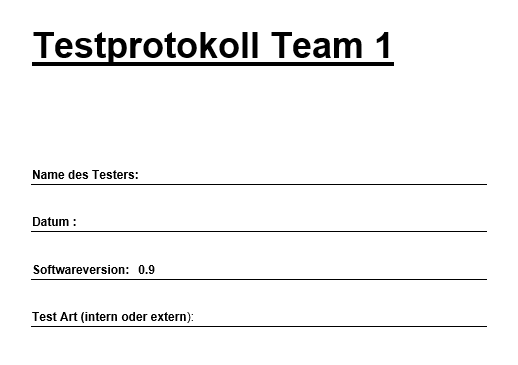
\includegraphics[width=16cm]{Protokoll.png}
	\label{fig:Protokoll}
\end{figure}

\begin{figure}[H]
	\centering
	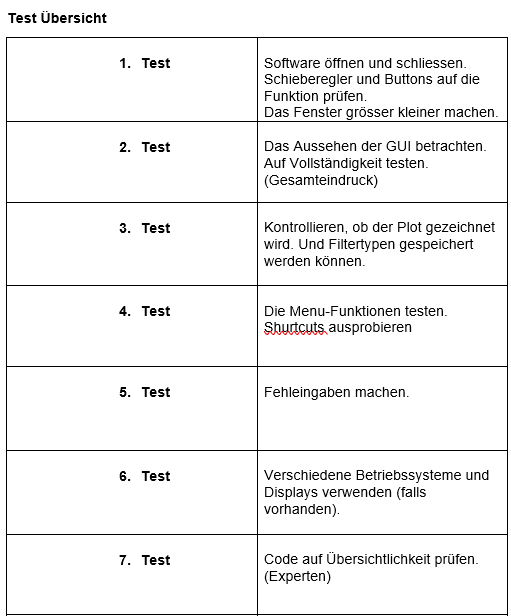
\includegraphics[width=16cm]{uebersicht.png}
	\label{fig:übersicht}
\end{figure}

\begin{figure}[H]
	\centering
	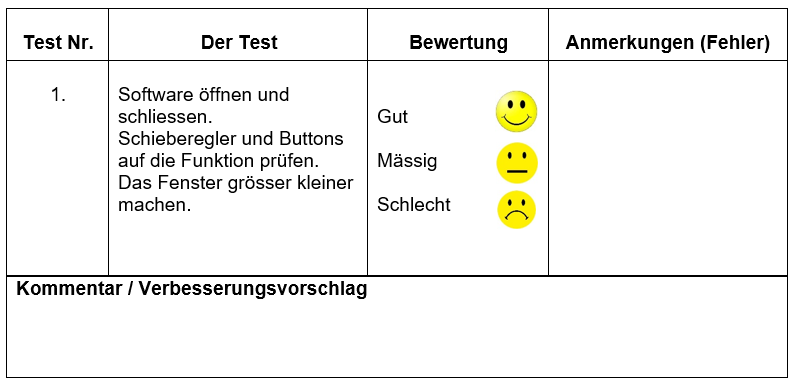
\includegraphics[width=16cm]{Test1.png}
	\label{fig:Test1}
\end{figure}

\begin{figure}[H]
	\centering
	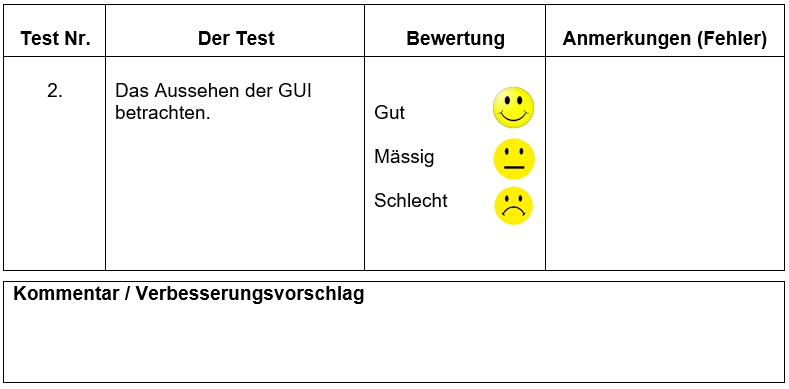
\includegraphics[width=16cm]{Test2.png}
	\label{fig:Test2}
\end{figure}

\begin{figure}[H]
	\centering
	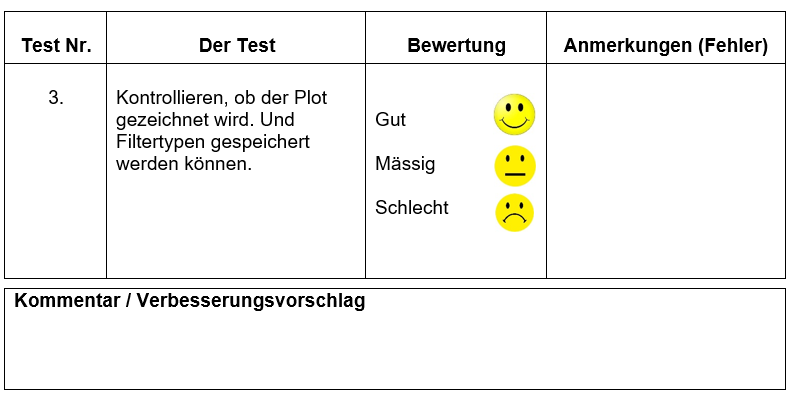
\includegraphics[width=16cm]{Test3.png}
	\label{fig:Test3}
\end{figure}

\begin{figure}[H]
	\centering
	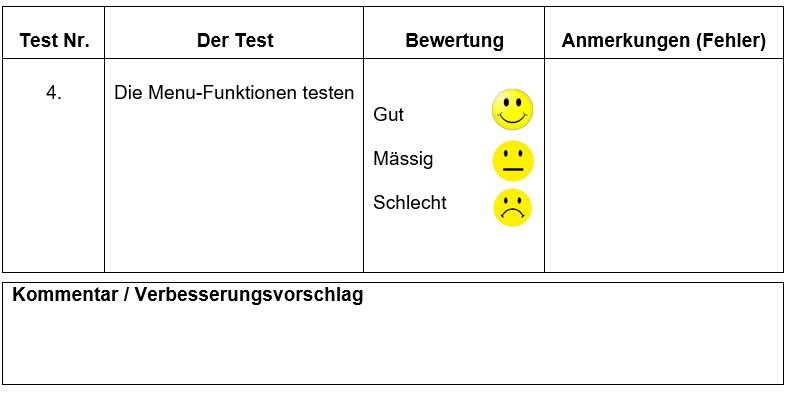
\includegraphics[width=16cm]{Test4.png}
	\label{fig:Test4}
\end{figure}

\begin{figure}[H]
	\centering
	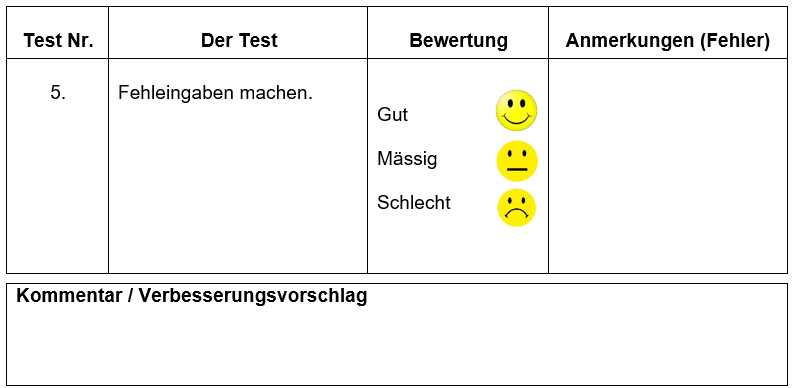
\includegraphics[width=16cm]{Test5.png}
	\label{fig:Test5}
\end{figure}

\begin{figure}[H]
	\centering
	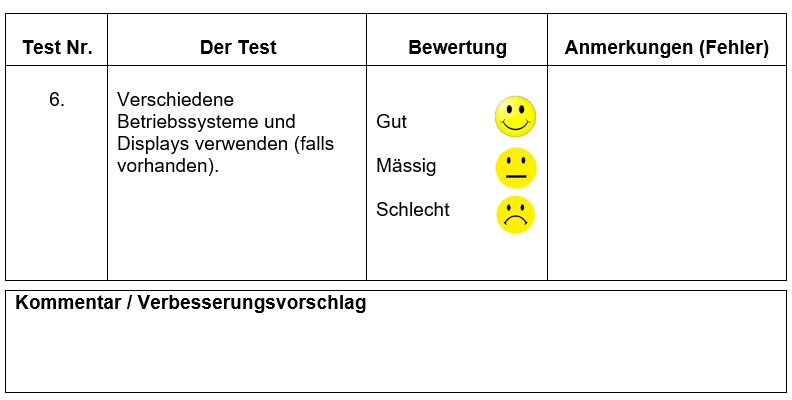
\includegraphics[width=16cm]{Test6.png}
	\label{fig:Test6}
\end{figure}

\begin{figure}[H]
	\centering
	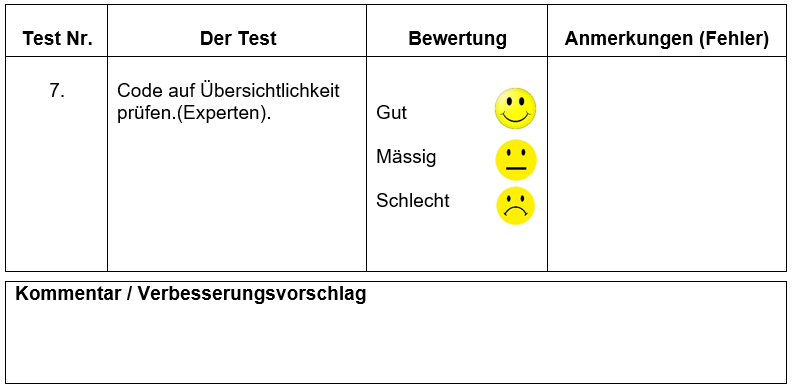
\includegraphics[width=16cm]{Test7.png}
	\label{fig:Test7}
\end{figure}

\begin{figure}[H]
	\centering
	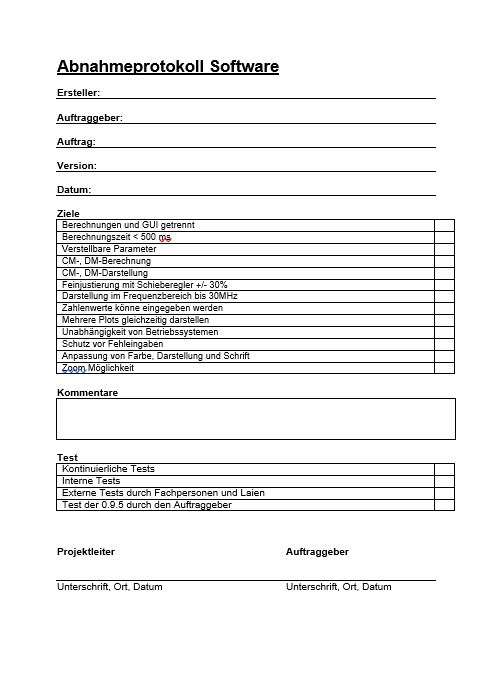
\includegraphics[width=16cm]{Abnahme.png}
	\label{fig:Protokoll}
\end{figure}

%%---NOTES for DEBUG---------------------------------------------------------------------
\ifdraft{%Do this only if mode=draft
%%requires \usepackage{todonotes})
\newpage
\listoftodos[\section{Todo-Notes}]
\clearpage
}
{%Do this only if mode=final
}
\end{document}
